%!TEX root = D2.1_AMIDSTModellingFramework.tex


\newpage
\newpage
\newcommand{\X}{\mathbf{X}}
\newcommand{\Y}{\mathbf{Y}}
\newcommand{\Z}{\mathbf{Z}}
\newcommand{\x}{\mathbf{x}}
\newcommand{\argmax}[1]{\underset{#1}{\operatorname{arg}\,\operatorname{max}}\;}


\subsection{CajaMar Models}
\label{Section:CajaMarModels}

\subsubsection{Introduction}

There are two tasks to be solved for Cajamar's Use Case~\cite{Fer14b}. The main one is the estimation of the \emph{probability of default}, defined as the probability that a
customer will end up as defaulter within the next two years. The second task consists in obtaining good customer profiles in terms of risk, so that marketing campaigns can be specifically targeted to these low risk customers. 

%-------------------------------------------------------------------------------------------------------
\subsubsection{Predicting probability of default} \label{SubSection:Predicting}
%-------------------------------------------------------------------------------------------------------

In any commercial bank, every time a customer applies for a loan, the bank experts evaluate the customer's risk profile before making their decision. 

At Cajamar, this risk evaluation protocol is addressed by evaluating whether the client is going to default or not within the following two years. When a client is labelled as defaulter, he/she will remain defaulter in the database at least for two more years. Then, the client could become non-defaulter again when everything has been appropriately paid during the last 2 years. 

The problem of predicting the risk of default is currently solved at Cajamar by an automatic supervised classification model (i.e., a logistic regression). It takes information about the recent financial activity of a customer, as well as information about recent past payment behaviour provided by other Spanish financial institutions. Finally, using this collected information, the probability that the client will default during the following two years is computed. 

The methodology currently employed does not assume any dependence structure among the variables, and current predictions are made using only $27$ variables out of more than $1000$ variables available. Updates in risk predictions are made on a monthly basis, whereas the predictive model is only updated after several years. These low update frequencies are partly due to limitations in the available commercial software and the computing resources.

Our objective is to \textit{daily} update the risk of default for every bank customer. This daily evaluation will be performed using two data sets: \textit{the model training data set} and \textit{the model evaluation data set} (see~\cite{Fer14b}). How these data sets are generated gives us some insights into the nature of this risk prediction problem. Figure~\ref{Figure:CajaMarTimeLine} illustrates how both evaluation and training data sets are collected within a time-line. The current time is denoted as $t$ and the time $2$ years back as $k$, i.e., $k=t-2$ years. 

\begin{figure}[htbp]
\centering
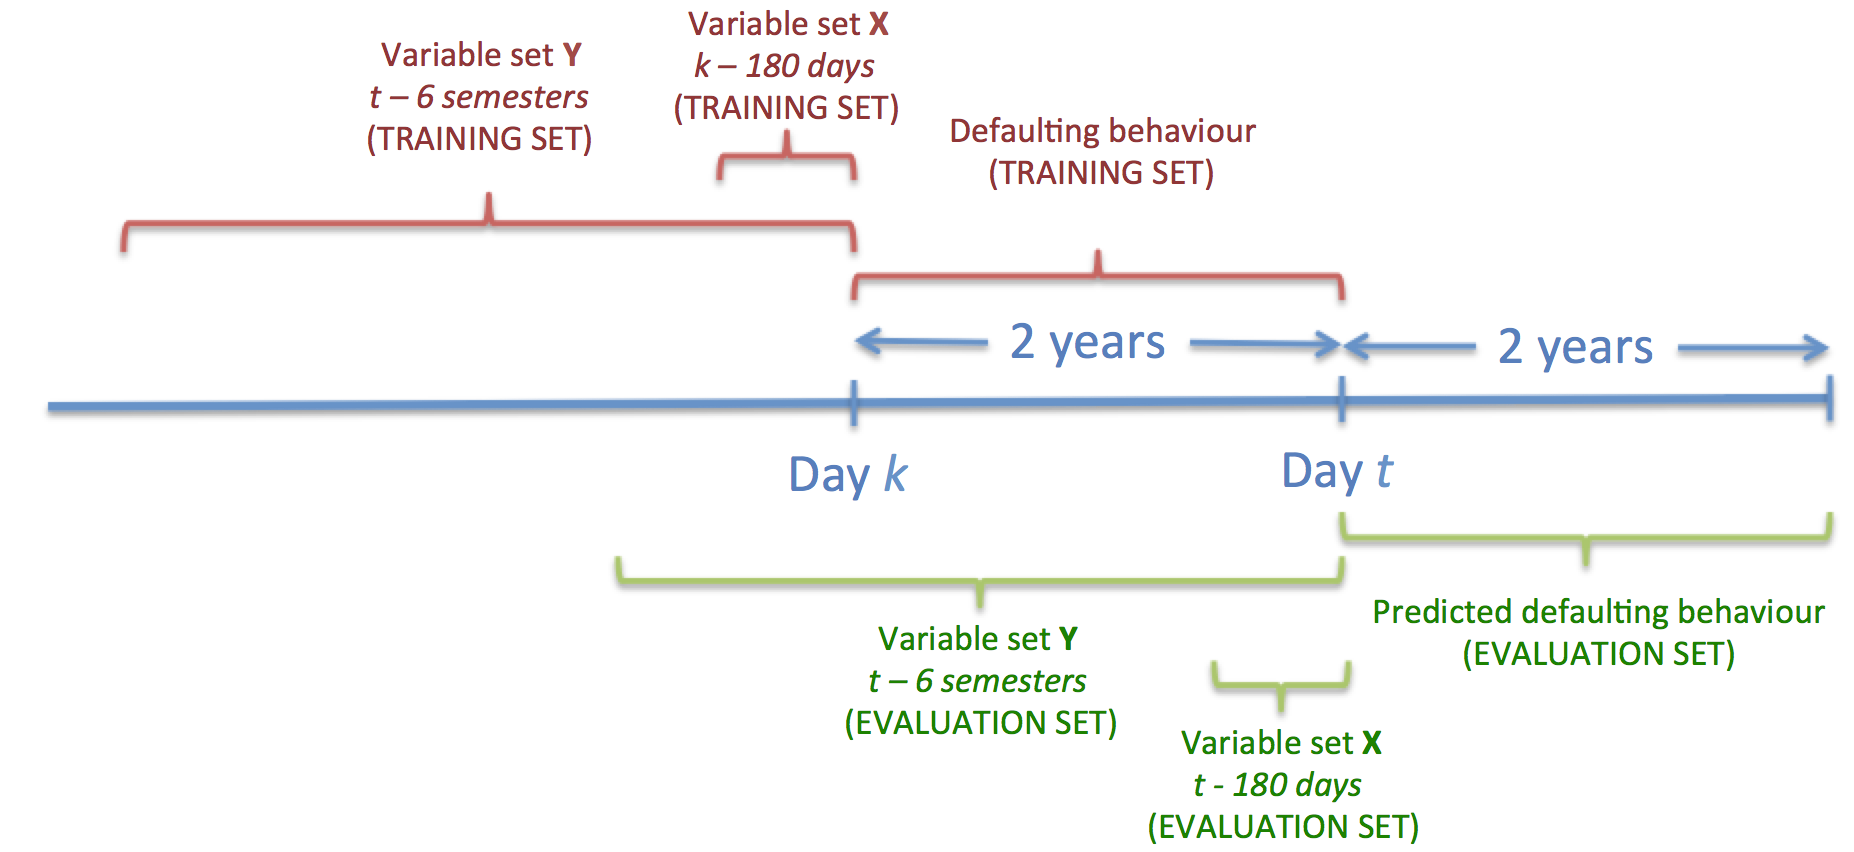
\includegraphics[scale=0.65]{figures/CajaMarTimeLine}
\caption{\label{Figure:CajaMarTimeLine}Time-line showing how the evaluation and training data sets are generated.}
\end{figure}

\begin{itemize}

\item \textbf{Model evaluation data set:} This data is created at time $t$ and contains a record for every client to be evaluated. Note that, information about the predicted defaulting behaviour is still missing at time $t$ when conforming the evaluation dataset. This information will be obtained after performing inference on the model. Predictive variables refer here to the financial activity and payment behaviour of the customers in recent past as well as to their socio-demographic information which usually does not change over time.

The recent {\bf financial activity} of a customer refers to attributes such as ``account balance'', ``number of credit card operations'', etc. stored in the last 180 days\footnote{This limit is fixed by the Bank of Spain}. These attributes usually change daily for a customer, so they are encoded by introducing a set of variables for each attribute, one for each day back from the current time $t$. Hence, the financial activity of a customer is specified by a number of variables equal to 180 times the number of attributes. 

In the case of {\bf past payment behaviour}, the attributes refer to variables related to payments inside Cajamar (loans, mortgages, credits, etc.). Information from the last 36 months grouped by semester is considered for these variables. Therefore, a number of variables equals to $6$ times the number of attributes referring to the payment behaviour are used in this case. Moreover, some other static variables with information about payments to other financial institutions or companies (phone and electricity bill, public bodies, etc.) are included in this group of variables.

The dataset for the evaluation of customers is depicted in Table~\ref{tab:EvaluationDataset}. The group of variables denoted as $\Z$ mainly includes socio-demographic variables and they are not indexed over time as they remain fixed.  

\begin{table}[htbp]
\centering
\begin{tabular}{c|ccc|ccc|c}
	&\multicolumn{3}{c|}{Days} & \multicolumn{3}{c|}{Semester} \\
     Time $t$              & $\X^{(t-180)}$ & $\ldots$ & $\X^{(t-1)} $ & $\Y^{(t-6)}$  & $\ldots$ & $\Y^{(t-1)} $ & $\Z$  \\  
\hline
Client$_1$  &                                                  &              &                     &                               &                     &        \\ 
$\vdots$      &                                                 &               &                     &                                &                     &      \\ 
Client$_n$  &                                                &               &                     &                                &                     &     \\ 
\end{tabular}
\caption{Evaluation data set at time $t$. Predictive variables for financial activity, payment behaviour, and socio-demographic information are denoted as $\X$, $\Y$ and $\Z$, respectively. Current time is denoted as $t$}
\label{tab:EvaluationDataset} 
\end{table}

Finally, the objective is to compute the probability of defaulting within the following two years of each record (i.e., customer) from the evaluation data set, and afterwards update the risk table in the system (see Table~\ref{tab:riskTable}).

\begin{table}[h]
\centering
\begin{tabular}{c|ccc|ccc|c}
     Time $t$  & Risk of default \\  
\hline
Client$_1$  &    $r_1$  \\ 
$\vdots$      &   $\vdots$   \\ 
Client$_n$  &   $r_n$  \\ 
\end{tabular} 
\caption{Table containing the risk of defaulting for every client.}
\label{tab:riskTable}
\end{table}

If, at some point, the probability of default of a customer rises above a predefined threshold, the bank may take preventive actions to reduce the chances of defaulting by this customer.


\item \textbf{Model training data set:}  This data set is built in the same way as the evaluation data set. It contains the same set of predictive variables plus the \textit{Defaulter} variable. The main difference between both data sets is that they refer to different time points. In fact, the predictive variables in the evaluation data set are built from time $t$ (current time) backward, whereas the ones in the training data set are built from time $k$ (2 years before $t$) backward. The data set for training/updating the model is depicted in Table~\ref{tab:TrainingDataset}.
\begin{table}[h]
\centering
\begin{tabular}{c|ccc|ccc|c|c}
	&\multicolumn{3}{c|}{Days} & \multicolumn{3}{c|}{Semester} & \\
     Time $t$              & $\X^{(k-180)}$ & $\ldots$ & $\X^{(k-1)} $ & $\Y^{(k-6)}$  & $\ldots$ & $\Y^{(k-1)} $ & $\Z$ & Defaulter$^{(t)}$\\  
\hline
Client$_1$  &                                                  &              &                     &                               &                     &        &  \\ 
$\vdots$      &                                                 &               &                     &                                &                     &       & \\ 
Client$_n$  &                                                &               &                     &                                &                     &     & \\ 
\end{tabular} 
\caption{Training data set at time $t$ with $k=t - 2$ years.  The notation for predictive variables is the same as in Table~\ref{tab:EvaluationDataset}.}
\label{tab:TrainingDataset} 
\end{table}

As shown in Table~\ref{tab:TrainingDataset}, each record contains a class label indicating if the customer is defaulter or non-defaulter at time $t$ and the values for all predictive variables representing his financial activities, payment behaviour and socio-demographic informorlion. To decide if a customer is defaulter or not, we look at data 2 years back from the current time $t$. If during these two years, there is no evidence of defaulting and the client's payments (at Cajamar and other financial institutions) have been accomplished as expected, the client is labelled as non-defaulter. Otherwise, it is labelled as defaulter.
\end{itemize}

In what follows, we propose two modelling solutions for the risk prediction problem: static and dynamic.

%-------------------------------------------------------------------------------------------------------
\subsubsection*{Static model} 
%-------------------------------------------------------------------------------------------------------

In this first approach we do not explicitly consider some of the dynamics of the problem meaning that we do not model that a customer can be non-defaulter and defaulter at different times (e.g., a customer can be creditworthy and, after some time, go bankrupt due to unemployment). Instead, we consider a static prediction model that predicts whether the client will default or not within the next 2 years based on the financial behaviour of the client over a recent past. This is in fact similar to the current Cajamar prediction system. 

Figure \ref{Figure:CajaMarStatic} shows the general structure of the static model. The payment variables are grouped by semesters while the financial activity variables are grouped by day. Note that, past socio-demographic information are not necessary since it does not change frequently.

\begin{figure}[ht!]
  \centering
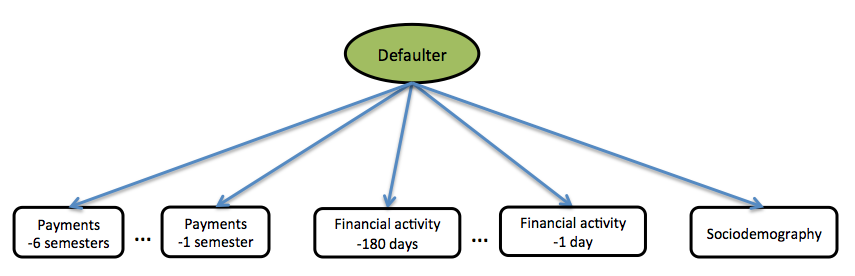
\includegraphics[scale=0.5]{./figures/CajaMarModel0}
\caption{\label{Figure:CajaMarStatic}Global structure of the static model. Each white box represents a set of variables for a particular time. The green node on top is the class variable \emph{Defaulter} that represents the probability that a customer will default within the next two years. } 
\label{fig:CajamarStaticModel}
\end{figure}

Expert knowledge from the bank pointed out that the predictive variables (mainly those within each white box) are expected to be related. Thus, in a first attempt we are assuming that only variables within each white box can be connected (e.g., according to a tree structure).

Another issue to consider is the possibility that one variable is a replica or contain quite similar information as another variable something expected in Cajamar's data. Consequently, their joint contribution will not only make learning and inference computationally more expensive, but it may also lead to a worse performance. This justifies the need to explore and use suitable feature selection techniques as specified in Use Case 2 of Cajamar's Requirement analysis~\cite{Fer14b}.

It is also of major interest to analyse the type of probability distributions to use in the proposed model. Figure \ref{Figure:cajamarMixt} shows the histograms for the values of one continuous predictive variable conditioned to defaulter (left curve) and non-defaulter (right curve) respectively. The resulting density curves represent a credible approximation using mixture of Gaussian distributions, which is the case for most of the remaining predictive variables. Note that, for defaulters, the values of the \emph{end-of-day balance} are overall lower compared to those corresponding to non-defaulters.

\begin{figure}[ht!]
  \centering
    \begin{tabular}{cc}
    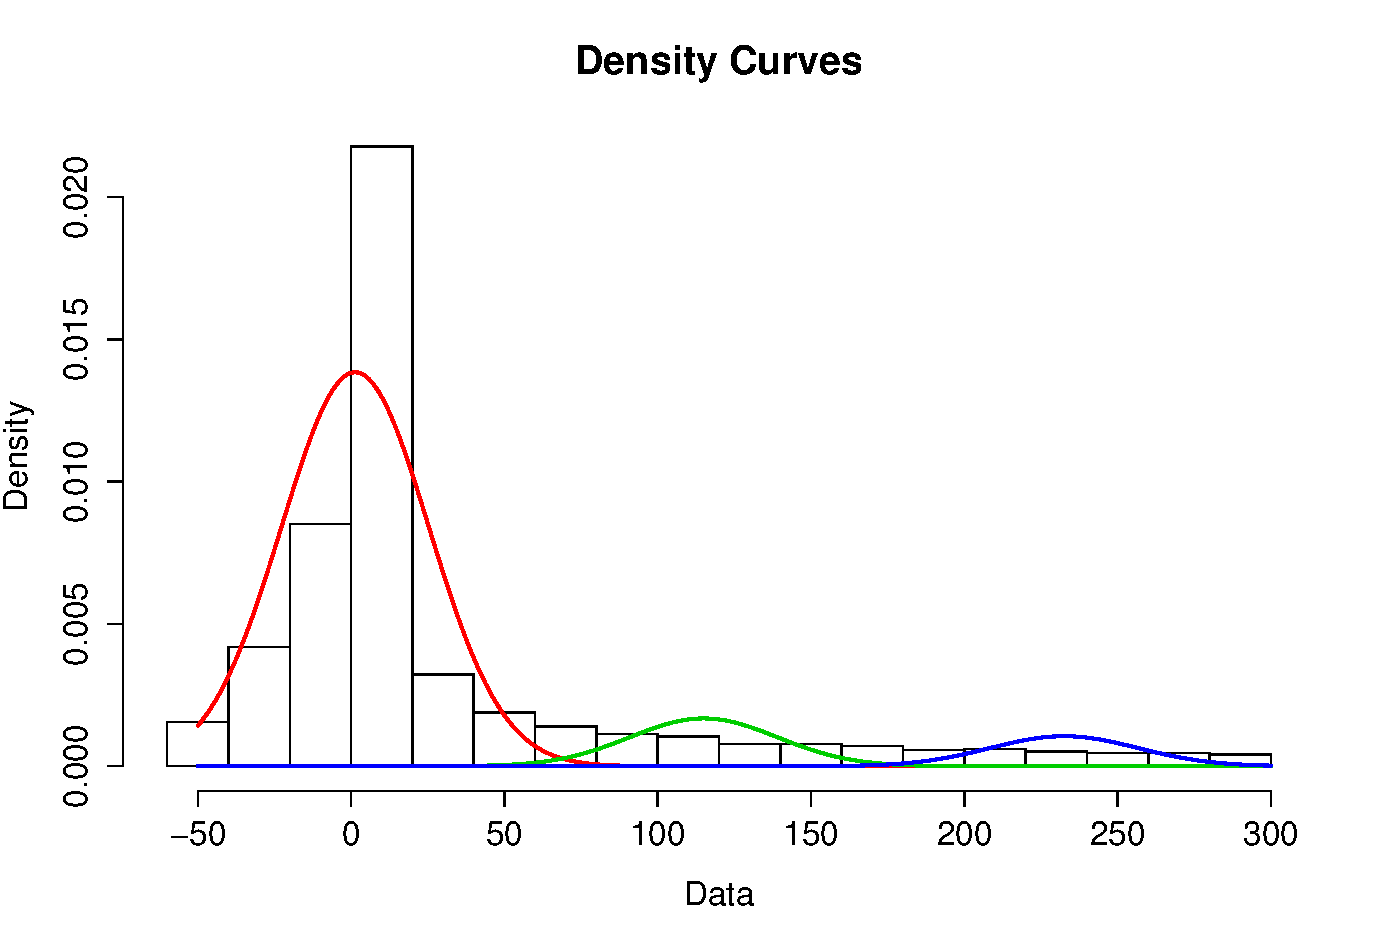
\includegraphics[width=70mm]{figures/CajaMarmixtureBalanceDef}&
    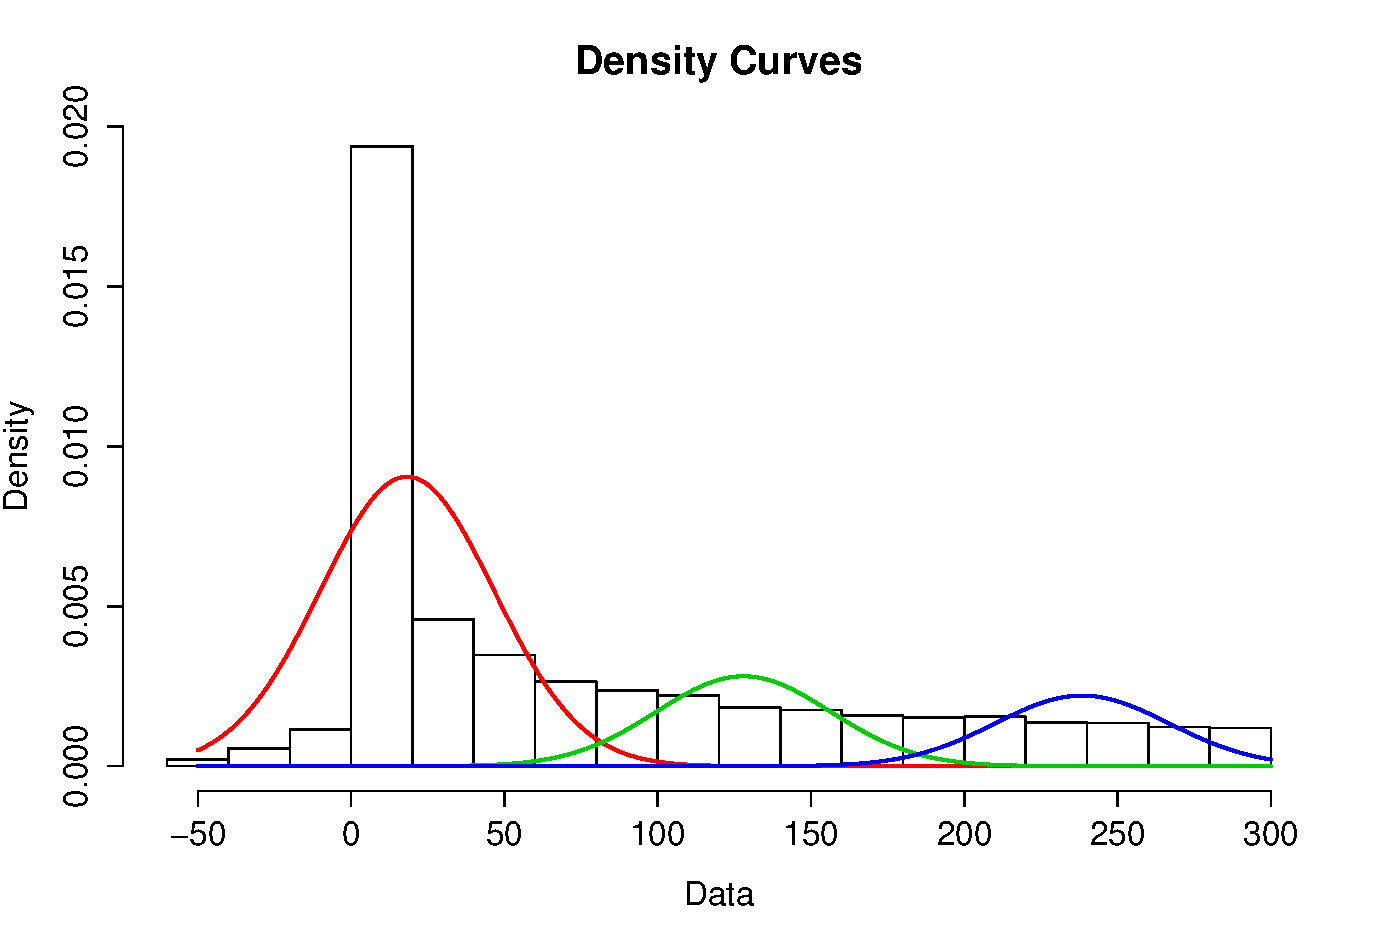
\includegraphics[width=70mm]{figures/CajaMarmixtureBalanceNonDef}\\
  \end{tabular}
    \caption{\label{Figure:cajamarMixt}Mixture of Gaussian approximations of one predictive variable conditioned to the class variable values defaulter (left) and non-Defaulter (right).}
\end{figure}

There exist however discrete (non-ordinal) predictive attributes which impose a limitation in the structure of the Conditional Gaussian network, since discrete attributes cannot have continuous parents as pointed out in Section~\ref{SubSection:HybridBNs}. This might not be a problem for the semi-naive Bayesian network to be considered, and it is certainly not a problem for naive Bayes. Nonetheless, if this limitation were found to be problematic, then other probability distributions families will be explored, such as Mixture of Truncated Basis Functions~\cite{Lan12}, which can cope with any generic model structure. 

In summary, the process of building the static model consists of the following steps:

\begin{enumerate}
\item Construct, every day, a single flat table containing the information for model training (see Table~\ref{tab:TrainingDataset}) using a set of SQL queries over the main relational data set. Note that, for instance, for variables related to financial activities, training data between two consecutive days $t$ and $t+1$ only differ in the new data arriving at day $t+1$ and obviating the data 180 days back from day $t$. Similar idea is applied for the payment behaviour variables.
\item Update the existing BN classifier with the new data. Although relationships are more common between variables within each box, dependences among variables in different boxes could be also considered. This possibility is tackled in Section~\ref{subsubsec:discussion}.
\item Construct a single flat table with the latest information about customers (evaluation data set as depicted in Table~\ref{tab:EvaluationDataset}) in order to compute the latest risk profiles. 
\item Update the risk in Table~\ref{tab:riskTable} for every customer by propagating each record from the evaluation data set on the static BN classifier obtained in Step 2. 
\end{enumerate}

%-------------------------------------------------------------------------------------------------------
\subsubsection*{Dynamic model} 
%-------------------------------------------------------------------------------------------------------

In this second approach, we will consider the dynamic structure of the problem because the behaviour of the customers evolves over time (e.g., the account balance is continuously changing from one month to another, the incomes, etc.) as well as their class labels either defaulters or non-defaulters (e.g., customers can be creditworthy and, after some time, go bankrupt because they have lost their job). 

Figure~\ref{fig:global_temp} represents the global idea of the proposed dynamic model. It can be compactly represented by a DBN made of components as the one displayed in 
Figure~\ref{fig:component}. $D_t$ represents the class variable at time slice $t$ (i.e., defaulting or non-defaulting client). Each feature variable with a clear dynamic component at time $t$, denoted as $X_t$, is linked to the same variable at time $t+1$, $X_{t+1}$. Although this is a reasonable assumption for most of the variables, this first Markov order relationship however might prove insufficient for some of the variables. Figure~\ref{fig:CajamarCorrelogramsAndPartial} show a partial correlogram and a correlogram for a continuous predictive variable (see Section~\ref{SubSubSection:StructuralAsumptions})\textcolor{red}{(include label in preliminaries section)}. The partial correlogram drop to almost zero for a lag equal to $2$, making a first Markov order assumption reasonable. However, a higher order could also rise from data, meaning that even earlier samples still could have an influence on the current sample given the previous one. 

$\bar{X}_{t-1}$ and $\bar{X}_{t}$ represents memory variables at time $t$ and $t+1$ respectively. The inclusion of this type of variables might be necessary when we have evidence that first order Markov relationships does not hold and we need to account for information coming from the past. For instance, a memory variable representing the average value during the last $180$ days could capture these dependences. Another reason to include these memory variables is that, even though they are computed from others, they provide information that might be disperse in the data and hardly can be captured with other variables as a whole. Another reason to use memory variables is to avoid building complex dynamic models with high Markov orders.

\begin{figure}[htbp]
\begin{center}
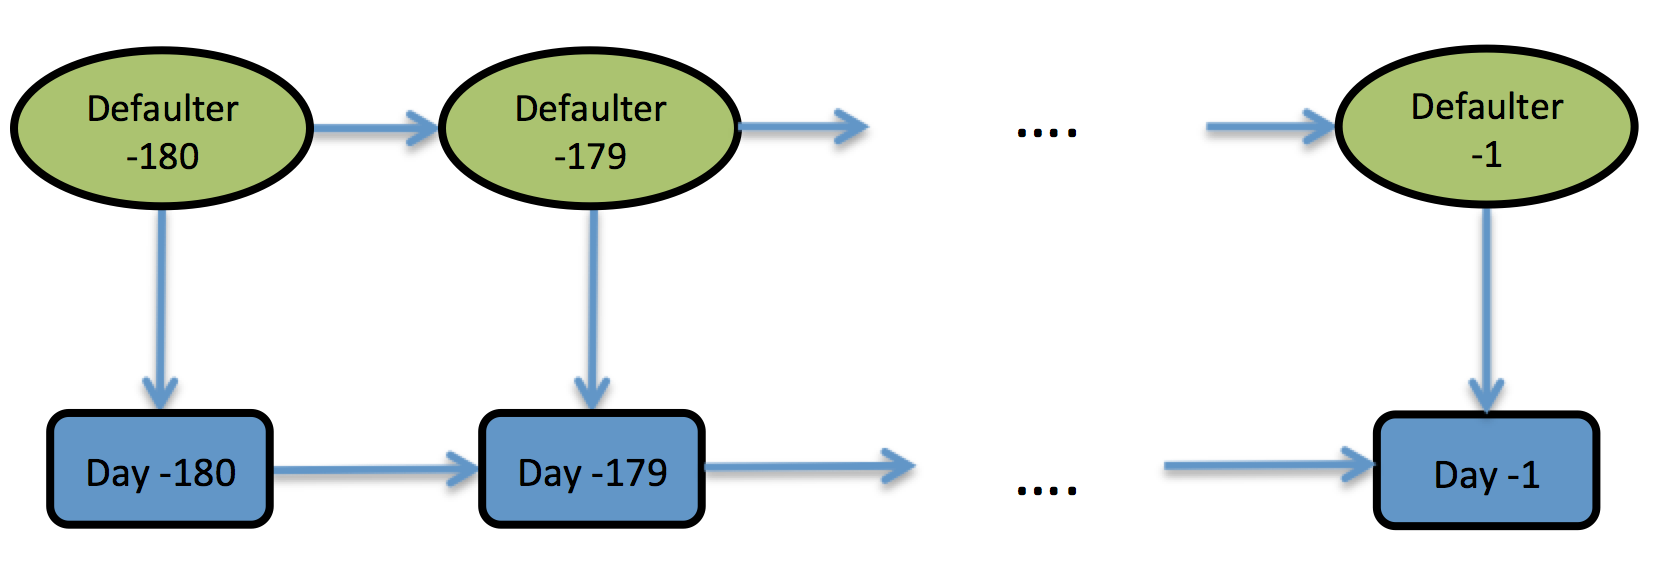
\includegraphics[scale=0.45]{./figures/CajaMarModel1}
\caption{Global structure of the dynamic model. Each white box represents a set of variables measured during the same day. The variables within a box can be connected as well as variables between two consecutive days representing the same attribute. For the ease of presentation, past payment behaviour and socio-demographic variables are omitted.}
\label{fig:global_temp}
\end{center}
\end{figure}


\begin{figure}[htbp]
\begin{center}
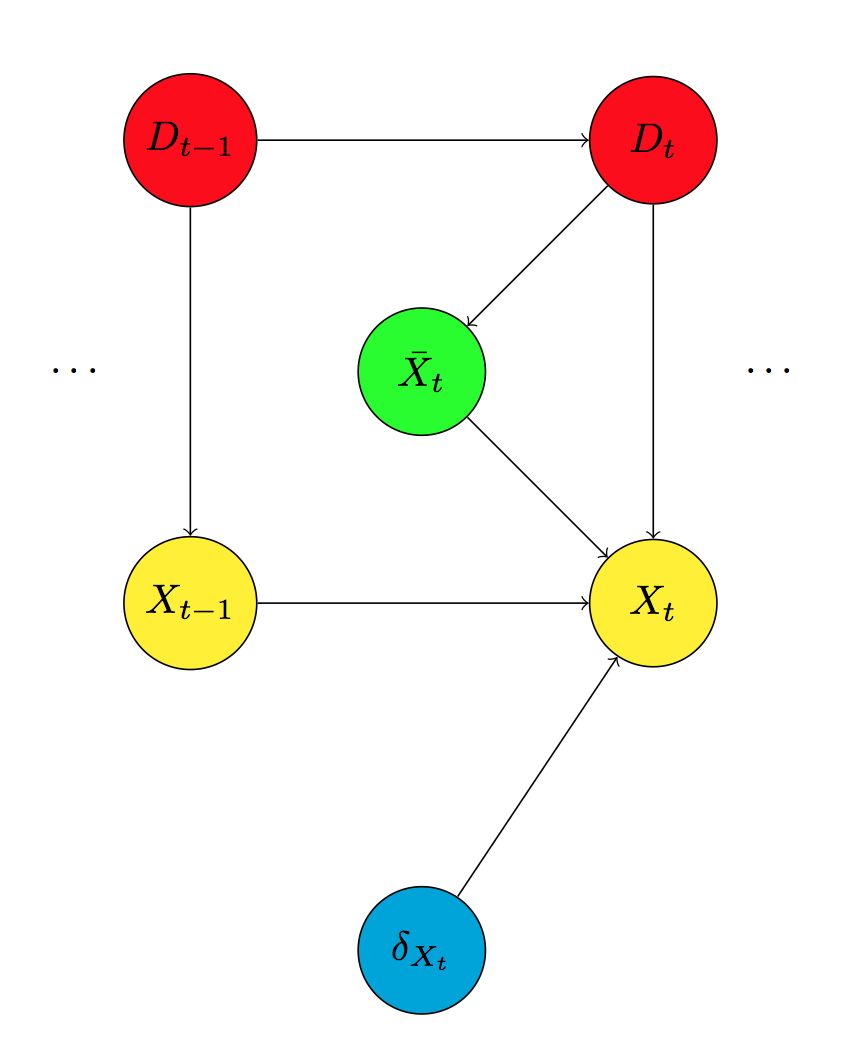
\includegraphics[scale=0.45]{./figures/CajaMarModel2}
\caption{Basic components of the DBN structure.}
\label{fig:component}
\end{center}
\end{figure}

\begin{figure}[htbp]
  \centering
   \begin{tabular}{cc}    
       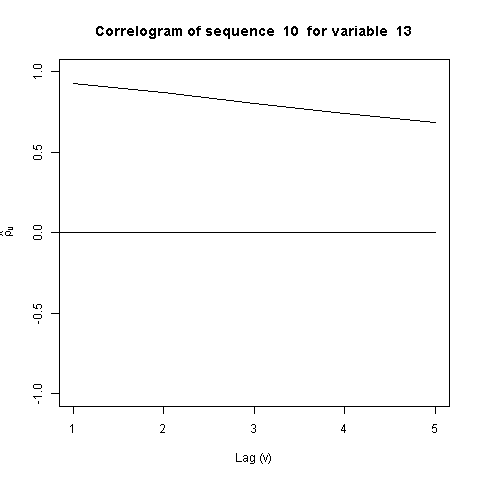
\includegraphics[width=70mm]{figures/CajamarCorrelogram} &
        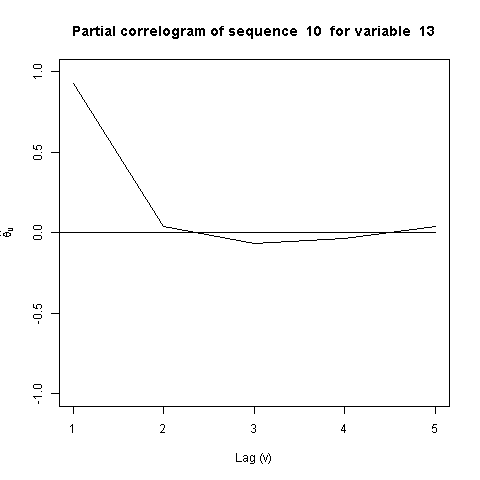
\includegraphics[width=70mm]{figures/CajamarPartialCorrelogram}
    \end{tabular}
     \caption{\label{fig:CajamarCorrelogramsAndPartial} Correlogram and partial correlogram for a variable. The x-axis represents the lag $v$ or time difference, and the y-axis represents the sample/partial autocorrelation coefficient of lag $v$, denoted $\hat{\rho_v}$ and $\hat{\delta_v}$, respectively (see Section \ref{Section:Preliminaries} for more details).}
\end{figure}

Another node included into the network is an indicator variable $\delta_{X_t}$, useful to model the situation in which a variable $X_t$ has a large number of zeroes, something that arises frequently in Cajamar's data. This is the case for every day payments made by credit card or the historical monthly outstanding amount on the account, for instance, whose value can be equal to zero for a large number of days for most customers. This fact affects seriously to learning because the real behavior of $X_t$ for values different from 0 is not adequately captured by the learnt distribution.
The solution is to use the indicator variable to condition the value of variable $X_t$ to $\delta_{X_t} = 0$ and $\delta_{X_t}\neq 0$. The indicator variables are not linked through consecutive time steps as only are used to indicate which data we model in the corresponding variable $X_t$. To better illustrate this, Figure \ref{fig:CajamarZeroes} (left) displays the histogram of a variable including all values, and Figure \ref{fig:CajamarZeroes} (right) displays the histogram of the same variable but excluding all zero values. Note that, the fitted density when zeros are discarded are extremely more representative than including zeros. This result undoubtedly justifies the use of the indicator variable $\delta_{X_t}$.

\begin{figure}[h]
  \centering
    \begin{tabular}{cc}    
       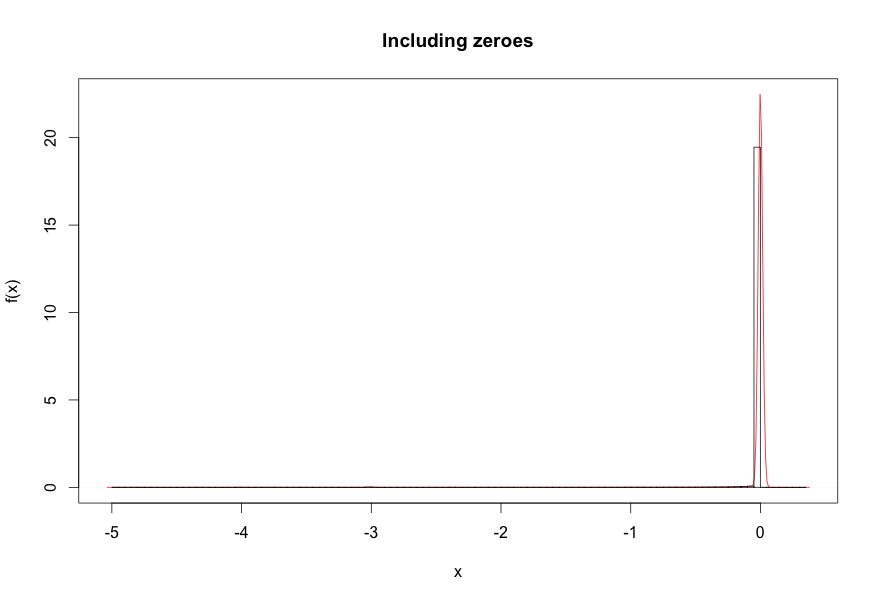
\includegraphics[width=70mm]{figures/with_zeroes}&
       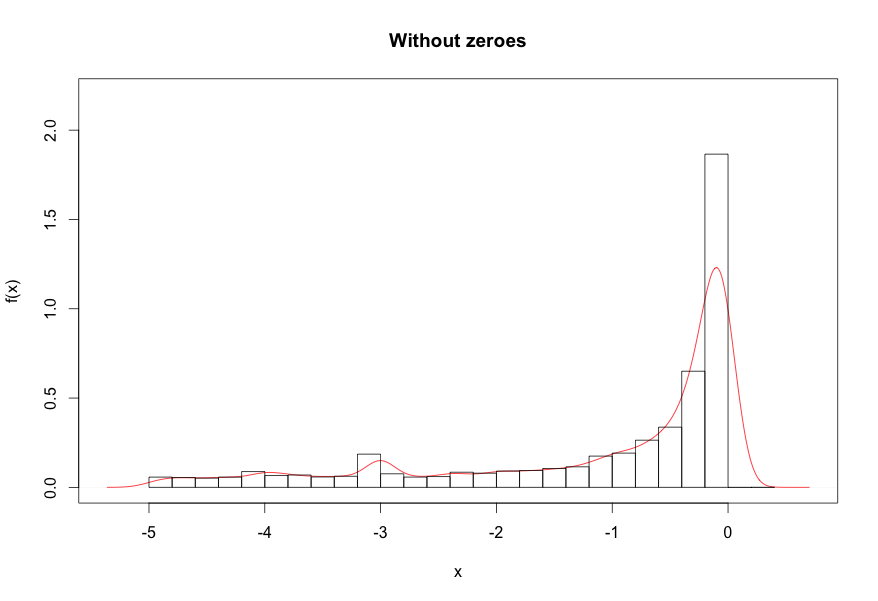
\includegraphics[width=70mm]{figures/without_zeroes}
    \end{tabular}
    \caption{\label{fig:CajamarZeroes}Data histograms and fitted densities for the same predictive variable including zero values (left) and discarding them (right).In both cases, outliers have been removed for a clearer representation}

\end{figure}

Finally, there exist some variables that, even though some dependences over time would be expected, they do not display any type of dynamic behaviour. For instance, this is the case for variables whose correllograms, shown in Figure \ref{fig:cajamarCorr}, indicate values very close to zero for all lags. These variables are hence not linked through consecutive time steps in the dynamic model, and are represented by $Y_{t+1}$ in Figure \ref{fig:component} together with the socio-demographic variables.

\begin{figure}[h]
  \centering
    \begin{tabular}{cc}
    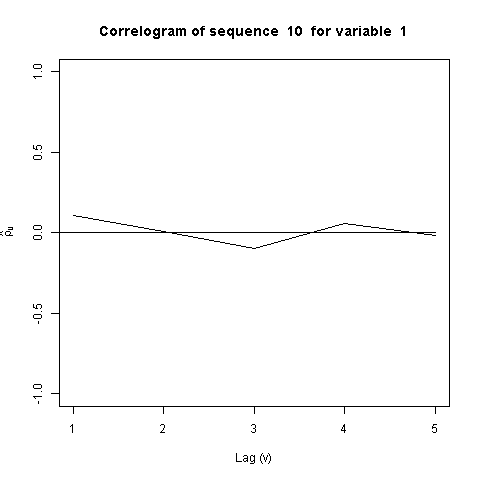
\includegraphics[width=70mm]{figures/CajaMarcrl1}&
     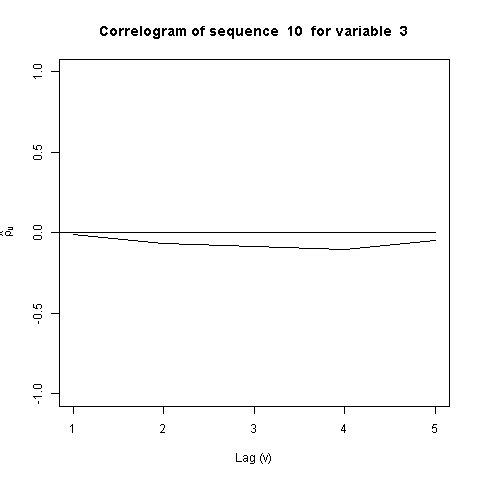
\includegraphics[width=70mm]{figures/CajaMarcrl3}\\
  \end{tabular}
    \caption{\label{fig:cajamarCorr}Example of correllograms for two predictive variables.  The x-axis represents the lag $v$ or time difference, and the y-axis represents the sample autocorrelation coefficient of lag $v$, denoted $\hat{\rho_v}$ (see Section \ref{Section:Preliminaries} for more details).}
\end{figure}


%-------------------------------------------------------------------------------------------------------
\subsubsection{Low risk profile extraction} \label{subsubsec:profileExtraction}
%-------------------------------------------------------------------------------------------------------

The marketing department at Cajamar periodically launches marketing campaigns for the recruitment of new products by customers (i.e., a new credit card, an insurance, etc.). The success of these campaigns depends greatly on the client group to which the campaign is targeted. It is also crucial to reduce as much as possible unnecessary expenses focused on non-potential customers. 

For this purpose, the marketing group proceeds as follows. First, they filter the customers based on their own marketing models and in collaboration with the risk department. Then, they select a subset of predictive variables considered relevant to be part of the final profile (mainly socio-demographic variables). For example, the age of a client is a relevant predictor when designing campaigns to attract customers for a death insurance. 

After obtaining the first group of customers for the campaign and determining the set of relevant attributes, the model proposed in Section~\ref{SubSection:Predicting} will be used to identify the profiles of the less risky clients using the most probable explanation (MPE) method~\cite{pearl1988probabilistic}. If we denote the \emph{Defaulter} variable as $D$ and  the set of predictors as $\X$, the idea to compute the assignment $\X = \x^{*}$ that has maximum a posteriori probability given the evidence $d=$ \texttt{no}, i.e., 

\begin{equation}
\x^{*} = \underset{\x\in\Omega_{\X}} {\mathrm{arg\,max}} ~ P(\x\mid d = \texttt{no})\, .
\label{eq:MPE}
\end{equation}

This procedure will be used to get the $k$ best MPEs or in other words the best profiles. Thus, the target customers previously filtered can be now grouped and ranked using these profiles which is really useful when designing the marketing campaigns.

%-------------------------------------------------------------------------------------------------------
\subsubsection*{Static model}\label{sec:StaticModel}
%-------------------------------------------------------------------------------------------------------

As pointed out before, mainly socio-demographic variables will determine the customer profiles used in the campaigns. These variables are mostly static as they do not change frequently over time (e.g., marital status, sex, type of job, ...). However, to enhance the analysis, a number of  variables changing over time will be included, although due to complexity reasons we should reduce this number as much as possible to make the profile extraction problem feasible.
The structure for the static model proposed in the profile extraction is the same as for predicting the risk of defaulting (see Fig.~\ref{fig:CajamarStaticModel}) but with a considerable reduction in the number of predictors used. 

For the profile extraction, the model not necessarily must have a classifier structure but it can have a general structure instead. However, what is desirable is to avoid using a NB structure for this task. The reason is that once the \emph{defaulter} variable is evidenced to \texttt{no}, the predictors become independent and the analysis would be poorer (MPE in this case would correspond to the maximum probability value for each variable individually).

%-------------------------------------------------------------------------------------------------------
\subsubsection*{Dynamic model}
%-------------------------------------------------------------------------------------------------------

As mentioned in Section~\ref{sec:StaticModel} the profile extraction problem mainly uses socio-demographic variables but in practice it might happen that variables related to financial activities or payment behaviour are required to be included in this model.  For instance, it could be of interest to include in a profile the tendency of a variable, i.e., the balance of a customer in the last days. For these reasons we should consider the modelling of a dynamic version for the profile extraction. 

The model for the profile extraction is the same as the one depicted in Figure~\ref{fig:component} but, as for the static approach, with a considerable reduction in the number of predictors. 
 
%-------------------------------------------------------------------------------------------------------
\subsubsection{Discussion and future models}\label{subsubsec:discussion}
%-------------------------------------------------------------------------------------------------------

The static and dynamic models presented above represent a first attempt to address the Cajamar use case. In this section, we will basically discuss the potential modifications and/or extensions that may occur in the subsequent phases of the AMIDST project to better meet Cajamar requirements presented in~\cite{Fer14b} or to face, for instance, other unexpected events.

The static model shown in Figure~\ref{fig:CajamarStaticModel} for predicting the probability of default is assumed to have only dependences among variables within each group of variables (white boxes). However, according to expert knowledge, no limitations should be imposed to the model structure among the predicting variables. Figure~\ref{fig:staticDependences} shows the modified structure of the static model when dependences among predicting variables are allowed, meaning that, variables within the dashed blue box could be connected as well. Note that, in this case, complexity grows considerably but, it is worth considering this approach to capture dependences that intuitively are not expected and therefore the analysis will be enriched.

\begin{figure}[ht!]
  \centering
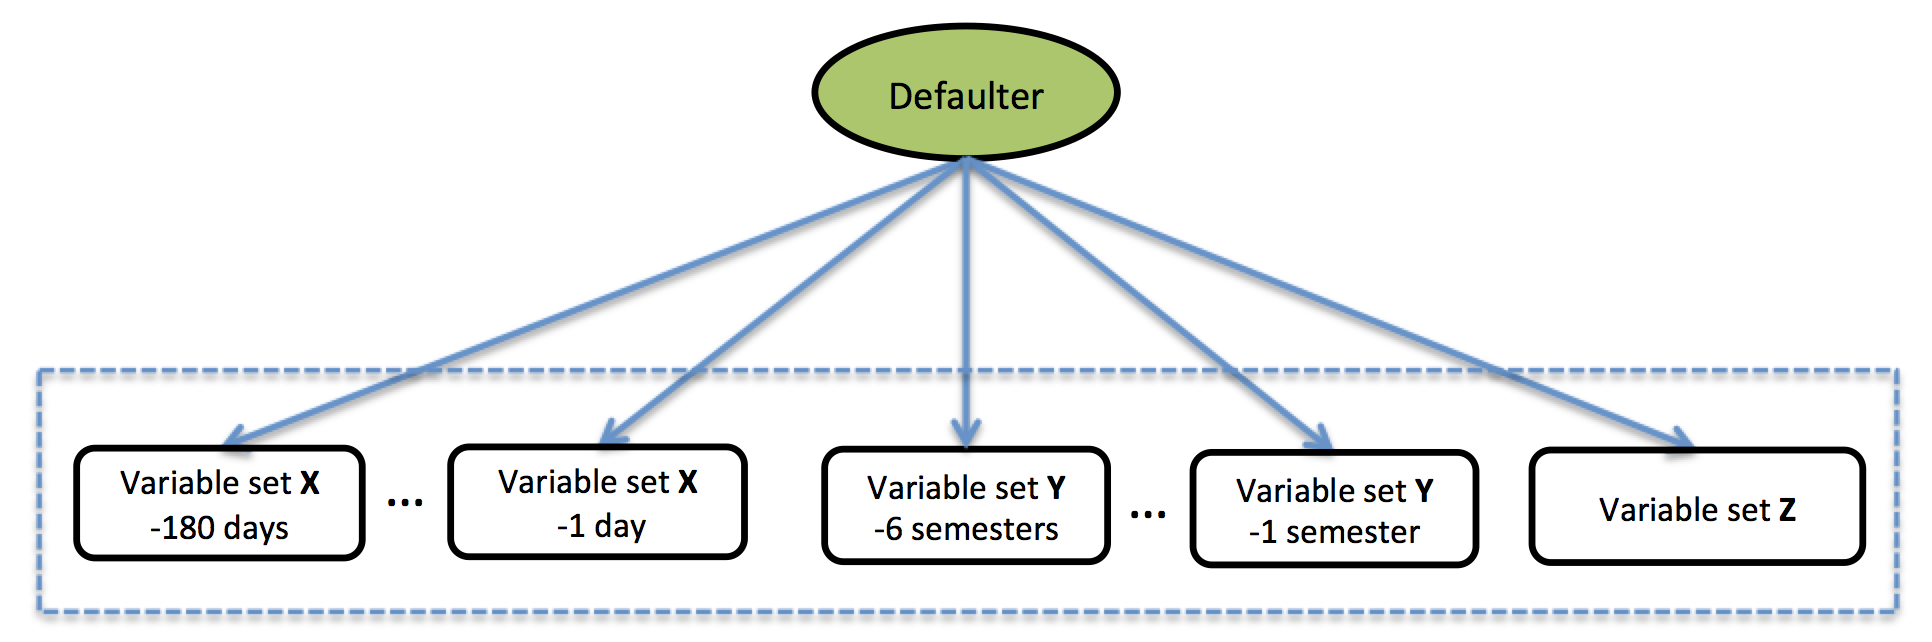
\includegraphics[scale=0.35]{./figures/CajaMarModel3}
\caption{\label{fig:staticDependences}Global structure of the static model allowing dependences among any variable within the dashed blue box. Each white box represents a set of variables for a particular time. The green node on top is the class variable \emph{Defaulter} that represents the probability that a customer will default within the next two years.} 
\end{figure}

In general, the model structure in Figure~\ref{fig:staticDependences} can not be modeled by CG distributions (see Section\ref{sec:}). If so, other probability distributions families will be explored. Mainly, they consist in translating the probability distribution into another such that learning and inference become feasible. These approaches include discretization or more complicated families based on Mixture of Truncated Basis Functions~\cite{Lan12}, which can cope with any generic model structure.

Another issue to be considered is about complexity in the profile extraction task explained in Section~\ref{subsubsec:profileExtraction}. It is well known that abductive inference over BNs and, in particular, the computation of the most probable explanations (MPEs) is an NP-hard problem~\cite{Shi94}. Thus, the model presented in Figure~\ref{fig:staticDependences}, which is valid for the profile extraction as well, could be simplified if necessary
by manually reducing the number of predictors in such a way that computational burden is adapted to the needs. In fact, this process is tightly connected to the expert knowledge provided by the marketing group, and this refinement would not be a problem.

The model for predicting the risk of default is assumed to be learnt every day. However, if required, this assumption can be relaxed and the learning process could be carried out less frequently. The results hardly will be affected as one-day data have little impact in comparison with the historical data captured in the current model so far. Note that, even if the model is not updated, the risk predictions are computed every day using the latest model available so far.